\SECTION{Design and Implementation}\label{sec:design_imple}
In this section, we present the design and implementation of Linux-RTXG,
which provides a framework of coordinated CPU and GPU resource
management with LKMs.
We describe our approach to GPU scheduling and its integration to CPU
scheduling.
Due to a space constraint, the detail of LKM-based CPU scheduling is
referred to the RESCH project~\cite{kato2009loadable, asberg2012exsched}.

\SUBSECTION{Linux-RTXG}
\begin{figure}[t]
\begin{center}
\ifthesis
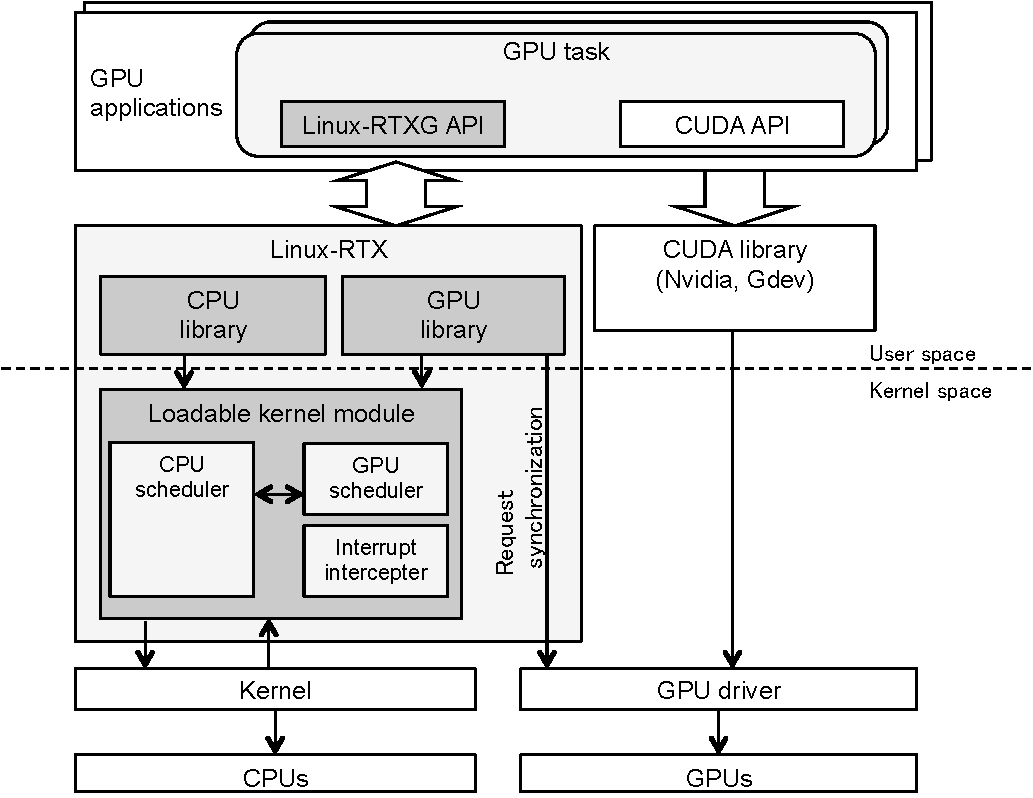
\includegraphics[width=0.8\textwidth]{img/overview.pdf}
\else
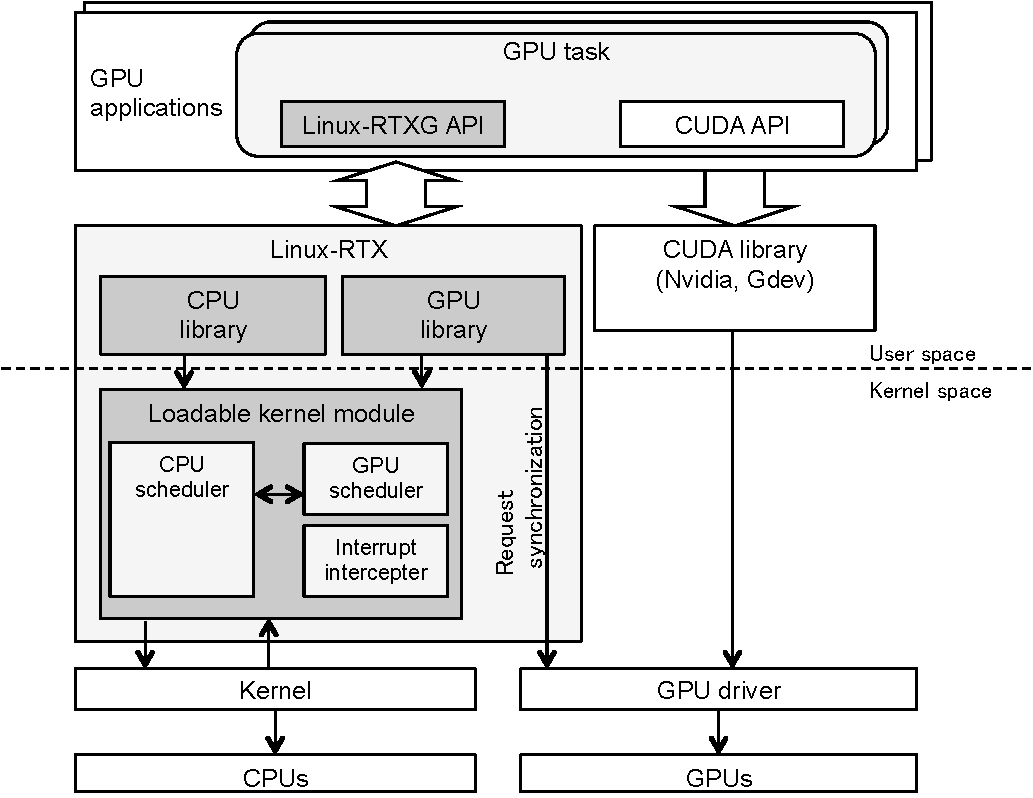
\includegraphics[width=0.35\textwidth]{img/overview.pdf}
\fi
\caption{Architectural overview of Linux-RTXG.}
\label{fig:overview}
\end{center}
\end{figure}

Figure~\ref{fig:overview} shows an architectural overview of
Linux-RTXG.
The system architecture of Linux-RTXG falls into two parts.
First, the Linux-RTXG core contains a CPU scheduler and a GPU scheduler
with a resource reservation mechanism.
The implementation of the Linux-RTXG core is provided in the kernel
space by an LKM.
Thus, it can use exported Linux kernel functions, such as $schedule()$,
$mod\_timer()$, $wake\_up\_process()$, and $set\_cpus\_allowed\_ptr()$.
These functions can be called from the user space interface using the
input/output control (ioctl) system call, which is a standard system
call for device drivers.
Secondly, the Linux-RTXG library contains an independent synchronization
method for coordinated CPU and GPU resource management.
The independent synchronization method can be used on top of a
proprietary driver~\cite{nvidia:cuda_zone} as well as an open-source
driver~\cite{nouveau}.
Note that this method is required to manage interrupts for GPU
scheduling without any code modification to the OS kernel and device
drivers.

\SUBSECTION{GPU Scheduling}
\begin{table*}[!t]
\begin{center}
\caption{A basic set of APIs for Linux-RTXG.}
\label{tab:rtx-api}
\ifthesis
\begin{tabular}{|l|p{25em}|} \hline
\else
\begin{tabular}{|l|p{50em}|} \hline
\fi
rtx\_gpu\_open() & Registers itself to Linux-RTXG and creates scheduling entity. It must be called first. \\ \hline
rtx\_gpu\_device\_advice() & Obtains recommendations for which GPU devices to use. \\ \hline
rtx\_gpu\_launch() & Controls GPU kernel launch timing, (i.e., a scheduling entry point). It must be called before the CUDA launch API. \\ \hline
rtx\_gpu\_sync() & Waits for the completion of GPU kernel execution by sleeping with TASK UNINTERRUPTIBLE status. \\ \hline
rtx\_gpu\_notify() & Sends NOTIFY/FENCE command to GPU. The FENCE/NOTIFY are selected by flag that is set by argument.\\ \hline
rtx\_gpu\_close() & Releases scheduling entity.\\ \hline
\end{tabular}
\end{center}
\end{table*}

Linux-RTXG is based on the interrupt-driven method for GPU
synchronization but is also partly based on the API-driven method.
The scheduler is invoked only when computation requests are submitted.
The basic APIs supported by Linux-RTXG are listed in Table~\ref{tab:rtx-api}.
Note that some APIs have arguments whereas others do not.
Linux-RTXG does not modify the existing CUDA API to cope with
proprietary software, being independent of GPU runtimes. 
However, CUDA application programs must add the Linux-RTXG APIs to use
the functionality of Linux-RTXG.

The sample code including the Linux-RTXG APIs is shown in
Figure~\ref{fig:sample}.
GPU tasks are provided with function calls to Linux-RTXG at strategic
points.

\begin{figure}[!t]
\begin{center}
\begin{tabular}{l}
\hline\hline
{\scriptsize \verb|void gpu_task(){        |}\\
{\scriptsize \verb| /* variable initialization  */        |}\\
{\scriptsize \verb| /* calling RESCH API */        |}\\
{\scriptsize \verb|  dev_id = rtx_gpu_device_advice(dev_id); |}\\
{\scriptsize \verb|  cuDeviceGet(&dev, dev\_id);           |}\\
{\scriptsize \verb|  cuCtxCreate(&ctx, SYNC_FLAG, dev);    |}\\
{\scriptsize \verb|  rtx_gpu_open(&handle, vdev_id);     |}\\
{\scriptsize \verb| /* Module load and set kernel function */ |}\\
{\scriptsize \verb| /* Device memory allocation        */ |}\\
{\scriptsize \verb| /* Memory copy to device from host */ |}\\
{\scriptsize \verb|  rtx_gpu_launch(&handle); |}\\
{\scriptsize \verb|  cuLaunchGrid(function, grid_x, grid_y); |}\\
{\scriptsize \verb|  rtx_gpu_notify(&handle); |}\\
{\scriptsize \verb|  rtx_gpu_sync(&handle);   |}\\
{\scriptsize \verb|  /* Memory copy to host from device */  |}\\
{\scriptsize \verb|  /* Release allocated memory */  |}\\
{\scriptsize \verb|}|}\\
\hline\hline
\end{tabular}
\caption{Sample code with the Linux-RTXG APIs.}
\label{fig:sample}
\end{center}
\end{figure}

\begin{figure}[!t]
\begin{center}
 \ifthesis
 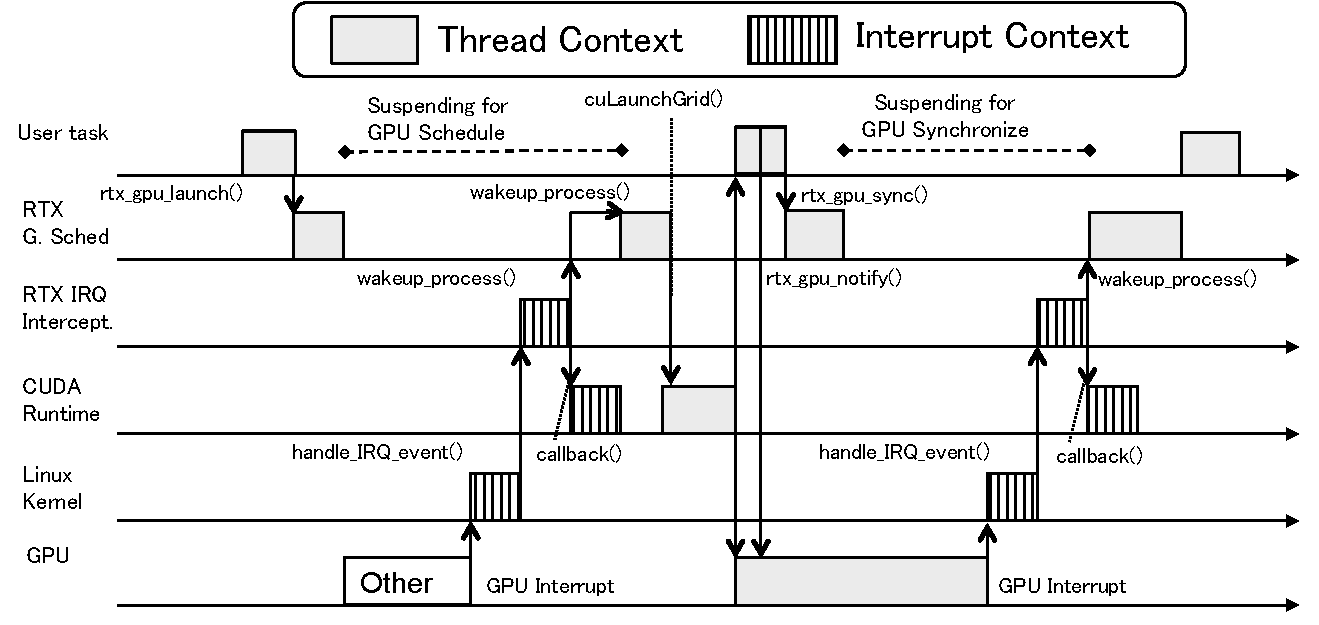
\includegraphics[width=\textwidth]{img/gsched_controlflow.pdf}
 \else
 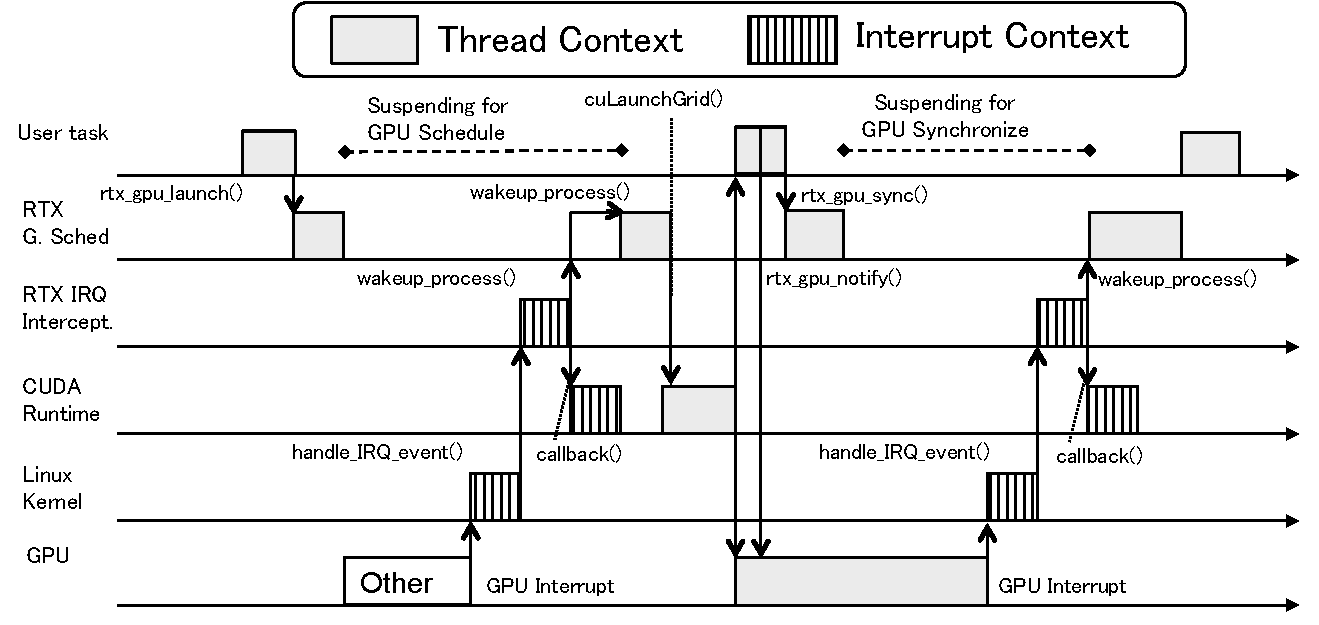
\includegraphics[width=0.5\textwidth]{img/gsched_controlflow.pdf}
 \fi
 \caption{Execution flow of the GPU task.}
 \label{fig:controlflow}
\end{center}
\end{figure}

The execution flow of the GPU task managed by the Linux-RTXG APIs is
described in Figure~\ref{fig:controlflow}.
Note that this example is restricted to a single GPU kernel.
The GPU task can control the timing of GPU kernel invocation by calling
$rtx\_gpu\_launch()$.
After this function call, the task is suspended until it receives an
interrupt so that other GPU kernels can be launched.
When some GPU kernel is completed, an interrupt is raised by the GPU and
the corresponding interrupt handler is executed by the Linux kernel.
The interrupt interceptor awakens some suspending task according to the
priority.
The awakened task proceeds to launch the GPU kernel using the CUDA API,
such as $cuLaunchGrid()$.
After the GPU kernel is launched, the task is going to register NOTIFY
to set up an interrupt, and is again put to the sleep mode until it
receives the interrupt.
Dispatching of the subsequent task is performed by the GPU scheduler,
which is called upon the interrupt from the GPU.
Linux-RTXG manages the order of task execution according to this flow.

We now present a hierarchal scheduling mechanism that uses the concept
of virtual GPUs to combine specified GPU tasks by a group.
The virtual GPUs are realized by a resource reservation mechanism, while
GPU scheduling uses a priority mechanism.
Specifically, each GPU kernel invocation is associated with a scheduling
entity, and Linux-RTXG allocates the scheduling entities to virtual GPUs. 
The virtual GPUs can belong to any physical GPUs.
In Linux-RTXG, computing resources are distributed to virtual GPUs.

Figure~\ref{fig:scheduling} shows the pseudo-code of the Linux-RTXG
scheduler.
This code works under the assumption that $on\_arrival$ is called when
some GPU task requests to launch the GPU kernel.
In $on\_arrival$, the GPU task checks whether the given execution
permission is held by the allocated virtual GPU and is also held by the
allocated scheduling entity.
If the virtual GPU to which the GPU task belongs does not own the
execution permission, the GPU task is enqueued to $wait\_queue$ and is
suspended.
Else, the GPU task can launch the GPU kernel.
After a while, $on\_completion$ is called by the scheduler thread when
the launched GPU kernel is completed, and we can select the next set of
a virtual GPU and a GPU task. 
At the end of $on\_completion$, the selected GPU task is waken up.

\begin{figure}[!t]
\begin{center}
\begin{tabular}{l}
\hline
{\scriptsize \verb| se: Scheduling entity |}\\
{\scriptsize \verb| se->vgpu: Group that belongs to se|}\\
{\scriptsize \verb| se->task: Task that is associated with se |}\\
{\scriptsize \verb| vgpu->parent: Physical GPU identifier|}\\
\hline
{\scriptsize \verb|void on_arrival(se) {|}\\
{\scriptsize \verb| check_permit_vgpu(se->vgpu)    |}\\
{\scriptsize \verb| while(!check_permit_se(se)){|}\\
{\scriptsize \verb|   enqueue(se->vgpu,se); |}\\
{\scriptsize \verb|   sleep_task(se->task); |}\\
{\scriptsize \verb| }|}\\
{\scriptsize \verb|}|}\\
{\scriptsize \verb|void on_completion(se) {|}\\
{\scriptsize \verb| reset_the_permit(se->vgpu, se)|}\\
{\scriptsize \verb| n_vgpu = pick_up_the_next_vgpu(se->vgpu->parent) |}\\
{\scriptsize \verb| se = pick_up_the_next_se(n_vgpu)|}\\
{\scriptsize \verb| if(se) {|}\\
{\scriptsize \verb|   dequeue(se->vgpu,se);|}\\
{\scriptsize \verb|   wakeup_task(se->task);|}\\
{\scriptsize \verb| }|}\\
{\scriptsize \verb| set_the_permit(se->vgpu, se)|}\\
{\scriptsize \verb|}|}\\
\hline
\end{tabular}
\caption{High-level pseudo-code of the Linux-RTXG scheduler.}
\label{fig:scheduling}
\end{center}
\end{figure}

\SUBSECTION{GPU Synchronization}
We next describe the independent synchronization mechanism and the
interrupt interception approach.
The independent synchronization mechanism invokes NOTIFY and FENCE
without using the GPU runtime API.
The interrupt interception enables interrupt-driven invocation of the
scheduler without making any modification to the OS kernel and device
drivers.
By this means, Linux-RTXG does not require to modify the OS kernel and
device drivers, while being able to create the scheduling points for GPU
tasks. 

\textbf{Independent Synchronization Mechanism:}
We now present the independent synchronization mechanism using NOTIFY
and FENCE.
This mechanism invokes an interrupt using NOTIFY, and writes the fence
value using the GPU microcontrollers and FENCE.
NVIDIA's proprietary software uses the ioctl interface to communicate
with the kernel space and the user space. 
These ioctl interfaces provide driver functions, such as device memory
allocation, obtaining GPU states and memory mapping. 
Gdev contains a runtime library that can control the GPU on top of
NVIDIA's proprietary driver using these ioctl interfaces. 
Our mechanism also uses an ioctl interface similar to Gdev in order to
send commands to the GPU.
Specifically, our mechanism is divided into two parts, (i)
initialization and (ii) notification.

The initialization process generates a dedicated GPU context.
This process creates virtual address space, allocates an indirect buffer
object for commands, and creates a context object that is required to
employ the FIFO engine, followed by the allocation of a kernel memory
object and the mapping of the FIFO engine registers to host memory space
through memory-mapped I/O (MMIO). 
The FIFO engine is a GPU microcontroller that decodes and dispatches the
commands sent from the host CPU side.

The notification process sends commands to a GPU compute engine or a GPU
data-copy engine by the $iowrite$ function associated with the mapped
FIFO engine registers so that an interrupt will be raised from the GPU
to the CPU.
The compute engine and the data-copy engine are such GPU
microcontrollers that control the states of GPU computation and data
transfer.
They are also used to switch GPU contexts on the GPU computation and
data transfer.
Note that this independent synchronization mechanism requires the
information of ioctl interfaces.
Therefore, it depends on the GPU architecture and implementation of
device drivers.

\textbf{Interrupt Interception:}
Interrupts are handled by the ISR that is registered to the Linux kernel
by the device driver.
The scheduler function is required to receive the interrupts and
identify them by reading the GPU status register.
The GPU status register must be read by the OS scheduler before it is
reset by the ISR.

The Linux kernel has a structure that holds interrupt parameters called
$irq\_desc$ for each interrupt number.
This structure has an internal structure called $irq\_action$,
including the ISR callback pointer.
The $irq\_desc$ structure is allocated to the global kernel memory
space, and is freely accessible from the kernel space.
Therefore, not only the Linux kernel but also external LKMs can obtain
the information of $irq\_desc$ and the ISR callback pointer.
We obtain the ISR callback pointer associated with the GPU device
driver, and register a new interrupt interception ISR to the Linux
kernel.
Finally, we can intercept interrupts from the GPU through the ISR and
retain the callback pointer.
In addition, I/O registers are mapped to the kernel memory space by the
device driver from the PCIe base address registers
(BAR)~\cite{fujii:icpads2013,kato2013zero}.
Therefore, Linux-RTXG remaps the BAR0 to our allocated space using
$ioremap()$ when the ISR is initialized. 
The interrupt interception mechanism can identify the source of every
interrupt by reading this remapped space.

\SUBSECTION{Scheduler Integration}
The mainline Linux scheduler implements a few real-time scheduling
policies:
\begin{itemize}
 \item $SCHED\_DEADLINE$
 \item $SCHED\_FIFO$
 \item $SCHED\_RR$
\end{itemize}

$SCHED\_DEADLINE$ is the implementation of CBS and EDF, which is the
latest real-time scheduler for Linux introduced in the version 3.14.0,
while $SCHED\_FIFO$ and $SCHED\_RR$ represent fixed-priority
scheduling.
Unfortunately, synchronization does not work with the SCHED\_DEADLINE
scheduling policy for GPU tasks.
Let us describe two problems.
The first problem is attributed to the implementation of
$sched\_yield$.
Note that $sched\_yield()$ uses $yield()$ in the kernel space.
Releasing the CPU by $sched\_yield()$ while waiting for I/O in polling,
we can utilize CPU time more efficiently.
However, $sched\_yield$ will set the remaining execution time of the
polling task to zero by treating it as a parameter of $SCHED\_DEADLINE$.
As a result, the task cannot execute until the runtime is replenished in
the next period.
This means that $sched\_yield()$ should not be called while polling in
$SCHED\_DEADLINE$.
However, $sched yield()$ is frequently used by device drivers and
libraries.
Real-time performance of GPU computing, even in CUDA, could be affected
by this problem.
We address this problem by limiting the GPU synchronization method to
NOTIFY, eliminating the potential of FENCE, in the $SCHED\_DEADLINE$
scheduling policy.

The second problem is subject to the implementation of wake-up and sleep
functions, particularly the check equation~\ref{eq} when restoring a
task from the sleep state.
If the equation~\ref{eq} holds, the runtime is replenished and the
absolute deadline is set to the next cycle deadline.

{\scriptsize
\begin{equation}
\frac{Absolute\_Deadline - Current\_Time}{Remaining\_Runtime} > \frac{Relative\_Deadline}{Period} \label{eq}
\end{equation}
}

We revise this check condition so that the GPU execution time is
substracted from $Remaining Runtime$ when a task is restored by the GPU
kernel execution, except when a task is restored by the period.
